% Created 2021-01-24 Sun 22:48
% Intended LaTeX compiler: pdflatex
\documentclass[11pt]{article}
\usepackage[utf8]{inputenc}
\usepackage[T1]{fontenc}
\usepackage{graphicx}
\usepackage{grffile}
\usepackage{longtable}
\usepackage{wrapfig}
\usepackage{rotating}
\usepackage[normalem]{ulem}
\usepackage{amsmath}
\usepackage{textcomp}
\usepackage{amssymb}
\usepackage{capt-of}
\usepackage{hyperref}
\usepackage{minted}
\hypersetup{colorlinks=true, linkcolor=black, filecolor=red, urlcolor=blue}
\usepackage[turkish]{babel}
\author{Eren Hatırnaz}
\date{\today}
\title{Yazılım Gündemi - 2020/26 [TASLAK]\\\medskip
\large 29 Haziran - 5 Temmuz 2020 (Yayınlanmadı)}
\hypersetup{
 pdfauthor={Eren Hatırnaz},
 pdftitle={Yazılım Gündemi - 2020/26 [TASLAK]},
 pdfkeywords={},
 pdfsubject={},
 pdfcreator={Emacs 27.1 (Org mode 9.3)},
 pdflang={Turkish}}
\begin{document}

\maketitle
\shorthandoff{=}

\begin{center}
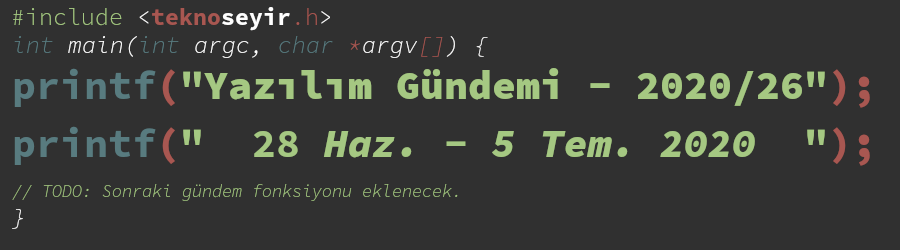
\includegraphics[width=.9\linewidth]{gorseller/yazilim-gundemi-banner.png}
\end{center}

\begin{center}
\href{../25/yazilim-gundemi-2020-25.pdf}{< Önceki Gündem} | \textbf{29 Haziran - 5 Temmuz 2020} |
\end{center}

\textbf{\textbf{Bu sayfa 2020 yılında yazmakta olduğum son Yazılım Gündemi yazısının taslak
halidir.}} \textbf{\textbf{Bu gündemde değerlendirilecek olan haberler aşağıdaki listedeki
bağlantılardır.}} \textbf{\textbf{Yazılım Gündemlerine ara vermeye karar verdiğim için bu şekilde
kaldı ama yine de bakmak isteyenler olabilir diye paylaşmak istedim.}}

\section*{Haberler}
\label{sec:orgd88165d}
\begin{itemize}
\item \href{https://about.gitlab.com/blog/2020/06/29/welcome-kde/}{Why the KDE community is \#MovingToGitlab | GitLab}
\item \href{https://godotengine.org/article/godot-40-gets-sdf-based-real-time-global-illumination}{Godot Engine - Godot 4.0 gets SDF based real-time global illumination}
\item \href{http://www.lua.org/manual/5.4/readme.html\#changes}{Lua 5.4 readme}
\item \href{https://github.com/vuejs/vue-next/releases/tag/v3.0.0-beta.16}{Release v3.0.0-beta.16 · vuejs/vue-next · GitHub}
\item \href{http://antirez.com/news/133}{The end of the Redis adventure - <antirez>}
\item \url{https://twitter.com/glenmaddern/status/1278252319646367744}
\item \href{https://codefund.io/}{CodeFund}
\item \href{https://security.googleblog.com/2020/06/system-hardening-in-android-11.html}{Google Online Security Blog: System hardening in Android 11}
\item \href{https://aws.amazon.com/tr/blogs/aws/aws-app2container-a-new-containerizing-tool-for-java-and-asp-net-applications/}{AWS App2Container – A New Containerizing Tool for Java and .NET Applications \ldots{}}
\item \href{https://github.blog/2020-07-01-launching-docs-github-com/}{Launching docs.github.com - The GitHub Blog}
\item \href{https://discourse.mozilla.org/t/common-voice-dataset-release-mid-year-2020/62938}{Common Voice Dataset Release - Mid Year 2020 - Common Voice - Mozilla Discourse}
\item \href{https://www.infoq.com/news/2020/07/mandrel-graalvm/}{RedHat Mandrel Makes Java Native}
\item \href{https://discourse.julialang.org/t/pkg-jl-telemetry-should-be-opt-in/42209}{Pkg.jl telemetry should be opt-in - Internals \& Design - JuliaLang}
\item \href{https://old.reddit.com/r/assholedesign/comments/hj57fv/apple\_forcing\_app\_developers\_to\_implement/}{Apple forcing app developers to implement auto-billing after free trial : ass\ldots{}}
\item \href{https://github.com/duckduckgo/Android/issues/527}{duckduckgo/Android\#527 Domains visited get leaked to DDG servers}
\item \href{https://devblogs.microsoft.com/python/announcing-pylance-fast-feature-rich-language-support-for-python-in-visual-studio-code/}{Announcing Pylance: Fast, feature-rich language support for Python in Visual \ldots{}}
\item \href{https://aws.amazon.com/tr/blogs/aws/find-your-most-expensive-lines-of-code-amazon-codeguru-is-now-generally-available/}{Find Your Most Expensive Lines of Code – Amazon CodeGuru Is Now Generally Ava\ldots{}}
\item \href{https://www.theregister.com/2020/07/01/mit\_dataset\_removed/}{MIT apologizes, permanently pulls offline huge dataset that taught AI systems\ldots{}}
\item \href{https://wiki.php.net/rfc/match\_expression\_v2}{PHP: rfc:match\_expression\_v2}
\end{itemize}
\section*{Lisans}
\label{sec:org287ef85}
\begin{center}
\begin{center}

\includegraphics[height=1.5cm]{../../../img/CC_BY-NC-SA_4.0.png}
\end{center}

\href{yazilim-gundemi-2020-26.pdf}{Yazılım Gündemi - 2020/26} yazısı \href{https://erenhatirnaz.github.io}{Eren Hatırnaz} tarafından \href{http://creativecommons.org/licenses/by-nc-sa/4.0/}{Creative Commons
Atıf-GayriTicari-AynıLisanslaPaylaş 4.0 Uluslararası Lisansı} (CC BY-NC-SA 4.0)
ile lisanslanmıştır.
\end{center}
\end{document}
